\section{Experiments}
\label{exp}
In Section \ref{exp}, we explain the experiment process in detail, including datasets, experimental setup, implementation details and evaluation results.

\subsection{Dataset}
\label{dataset}
Experiments are done on two datasets: FewRel dataset \cite{han-etal-2018-fewrel} and our proposed TinyRel-CM dataset.
~\\
~\\
\textbf{FewRel Dataset} FewRel dataset \cite{han-etal-2018-fewrel} is a few-shot relation classification dataset constructed through distant supervision and human annotation. It consists of 100 relation classes with 700 instances per class. The relation classes are split into subsets of size 64, 16 and 20 for training, validation and testing, respectively.
The average length of a sentence in FewRel dataset is 24.99, and there are 124,577 unique tokens in total. At the time of writing, FewRel is the only few-shot relation classification dataset available.
~\\
~\\
\textbf{TinyRel-CM Dataset}\footnote{Code and dataset released in \url{https://github.com/XiaoqingGeng/MICK}.} TinyRel-CM dataset is our proposed Chinese few-shot relation classification dataset in health domain with small training data. The TinyRel-CM dataset is constructed through the following steps: (1) Crawl data from Chinese health-related websites\footnote{\url{www.9939.com}, \url{www.39.net}, and \url{www.xywy.com}} to form a large corpus and an entity dictionary. (2) Automatically align entities in the corpus with the entity dictionary, forming a large candidate-sentence set. (3) 5 Chinese medical students manually filter out the unqualified candidate sentences and tag qualified ones with corresponding class labels to form an instance. An instance is added to the dataset only if 3 or more annotators make consistent decisions. This process costs 4 days.

The TinyRel-CM Dataset consists of 27 relation classes with 50 instances per class. The 27 relation classes cover binary relations among 4 entity types, and are grouped into 6 categories according to the entity types, forming 6 tasks with one group being the test set and other 5 groups serving as training set (see Table \ref{Egroup}). Grouping makes TinyRel-CM dataset more challenging because all candidate relation classes during testing are highly similar. An example instance in the TinyRel-CM dataset is shown in Tabel \ref{FRMexample}. The average length of a sentence in TinyRel-CM dataset is 67.31 characters, and there are 2,197 unique characters in total. Comparison between TinyRel-CM dataset and FewRel dataset is shown in Table \ref{Datasetcompare}.

\begin{table}[ht]
\centering
\small
\caption{Entity groups in TinyRel-CM dataset. D,S,F, and U stand for Disease, Symptom, Food, and nUtrient, respectively.}
\label{Egroup}
\begin{tabu}{|c|[0.5pt]l|}
\hline
\textbf{Group} & \textbf{Classes} \\ \tabucline[0.5pt]{-}
D-D & complication, cause, is, include, NA \\ \hline
D-S & have, NA\\ \hline
D-F & positive, negative, forbid, prevent, cause, NA\\ \hline
D-U & positive, negative, prevent, lack, cause, NA\\ \hline
F-U & contain, NA\\ \hline
S-F & forbid, cause, positive, negative, prevent, NA\\ \hline
\end{tabu}
\end{table}

\begin{table}[ht]
\centering
\small
\caption{An example instance in the TinyRel-CM dataset.}
\label{FRMexample}
\begin{tabular}{|l|p{170pt}|}
\hline
\textbf{Group} & D-D \\ \hline %\tabucline[1pt]{-}
\textbf{Class} & complication \\ \hline
\textbf{Explanation} & Entity 2 is a complication of entity 1. \\ \hline
\multirow{2}{*}{\textbf{Example}} & [子宫肌瘤]$_{entity1}$出现了[慢性盆腔炎]$_{entity2}$并发症,导致月经量过多。 \\
& \textcolor[rgb]{0.45,0.45,0.45}{Once [Hysteromyoma]$_{entity1}$ is complicated with [chronic pelvic inflammation]$_{entity2}$, menstruation increases.}  \\ \hline
\end{tabular}
\end{table}


\begin{table}[ht]
\centering
\small
\caption{Comparison of TinyRel-CM dataset to FewRel dataset.}
\label{Datasetcompare}
\begin{tabular}{|l|r|r|r|}
\hline
\textbf{Dataset} & \textbf{\#cls.} & \textbf{\#inst./cls.} & \textbf{\#inst.} \\ \hline
FewRel & 100 & 700 & 70,000 \\ \hline
TinyRel-CM & 27 & 50 & 1,350 \\ \hline
\end{tabular}
\end{table}


%The TinyRel-CM dataset is harder than FewRel dataset for two reasons. On one hand, the training data size is small (as is shown in Table \ref{Datasetcompare}). On the other hand, under each task, the candidate relation classes are relative to each other since they share common entity types (because the classes are from the same entity group). For example, a model needs to choose the correct relation class for the example instance in Table \ref{FRMexample} among classes \emph{Disease-complication-Disease, Disease-cause-Disease, Disease-is-Disease, etc.}.
%In FewRel dataset, the head and tail entity types are distinct in most of the cases (see Table~\ref{FewShotRCExample}), making the relation classes easier to distinguish.
%The difference in entity types may also
%%serve as extra information,
%mislead the models into learning to distinguish entity types instead of relation classes.
%%Figure xx shows example instances from previous datasets and the HEALTHXX dataset. For previous datasets, the instances within the same category is likely to be quite similar while instances from different categories distinct from one to another. While in HEALTHXX datasets, the format of instances within one category varies from one to another, which makes the task harder.

%
%\begin{table*}[hbt]
%\centering
%\tiny
%\begin{tabular}{|l|c|p{8pt}<{\centering}p{8pt}<{\centering}p{8pt}<{\centering}p{8pt}<{\centering}p{8pt}<{\centering}|p{8pt}<{\centering}p{8pt}<{\centering}p{8pt}<{\centering}p{8pt}<{\centering}p{8pt}<{\centering}|p{8pt}<{\centering}p{8pt}<{\centering}p{8pt}<{\centering}p{8pt}<{\centering}p{8pt}<{\centering}|p{8pt}<{\centering}p{8pt}<{\centering}p{8pt}<{\centering}p{8pt}<{\centering}p{8pt}<{\centering}|}
%\hline
%\multirow{3}{*}{\textbf{Method}} & \textbf{+} & \multicolumn{5}{c|}{\emph{- -}} &\multicolumn{5}{c|}{\emph{MME}} & \multicolumn{5}{c|}{\emph{Data}} & \multicolumn{5}{c|}{\emph{MME\&Data}} \\ \cline{2-22}
%& \multirow{2}{*}{\textbf{(N,K)}} & \multicolumn{20}{c|}{\textbf{Shrink origin training set size to }} \\ \cline{3-22}
%& &L0 &L1 &L2 &L3 & L4 & L0&  L1 &L2 &L3 & L4 &L0 & L1 &L2 &L3 & L4 & L0 & L1 &L2 &L3 & L4 \\ \hline
%\multirow{4}{*}{MetaN} & (~~5,1) &&&&& &&&&& &&&&& &&&&&\\
%& (~~5,5) &&&&& &&&&& &&&&& &&&&& \\
%& (10,1) &&&&& &&&&& &&&&& &&&&&\\
%& (10,5) &&&&& &&&&& &&&&& &&&&& \\ \hline
%\multirow{4}{*}{GNN} & (~~5,1) &61.87&53.95 &42.59 & 40.88&24.51   &63.20&55.81&46.85&40.61&23.09   &56.71&\textbf{58.40}&50.99&\textbf{51.92}&39.97    &\textbf{63.70} &56.83&\textbf{52.64}&48.26&\textbf{45.38}\\
%& (~~5,5)& 73.92&68.21 &55.16 & 52.24&28.94   &76.62&68.92&61.19&50.56&27.63    &70.76 &\textbf{71.96}&64.87&\textbf{66.17}&48.30     &\textbf{77.13} &71.42&\textbf{66.47}&60.94&\textbf{54.54}\\
%& (10,1) &53.32&38.57 &30.38 &28.08&18.91   &\textbf{54.87}&37.06&35.59&29.98&15.36    &54.81 &\textbf{43.99}&\textbf{37.64}&33.85&\textbf{30.32}     &54.23&42.53&36.98&\textbf{36.32}&29.36\\
%& (10,5) &65.64&52.07 &39.78 & 38.03&24.25   &67.15&51.41&47.91&41.05&20.03    &66.76 &\textbf{57.97}&50.33&47.74&\textbf{40.23}      &\textbf{67.80}&56.60&\textbf{50.85}&\textbf{49.73}&40.18\\ \hline
%
%\multirow{4}{*}{SNAIL} & (~~5,1) &29.85&\textbf{44.67}&33.36&33.64&20.85   &\textbf{48.25}&36.08&36.21&29.32&27.72     &30.82&42.40&35.38&35.32&28.26    &43.10&42.76&\textbf{39.70}&\textbf{39.08}&\textbf{34.32} \\
%& (~~5,5)&55.39 &53.62&46.66&38.41&28.81    &55.76&\textbf{61.36}&55.91&39.46&26.85     &\textbf{63.38}&57.74&48.68&43.70&20.02     &56.04&51.32&\textbf{56.44}&\textbf{44.04}&\textbf{38.28} \\
%& (10,1) &35.16&22.64&25.33&19.60&11.67    &35.43&\textbf{27.37}&24.07&24.65&15.72     &38.49&26.34&\textbf{27.19}&\textbf{28.00}&19.85     &\textbf{43.51}&26.52&25.85&27.77&\textbf{29.25}\\
%& (10,5) &47.73&36.40&\textbf{40.94}&\textbf{27.92}&13.08    &48.65&42.17&36.86&26.43&15.01     &\textbf{54.06}&37.36&31.92&23.51&25.57     &52.14&\textbf{42.18}&33.38&27.30&\textbf{26.34}\\ \hline
%
%\multirow{4}{*}{Proto} & (~~5,1) &71.50&67.94 &61.37 & 58.20&35.68   &71.44&66.98 &65.04 &59.25&40.04   &71.78&69.47&64.80&\textbf{64.48}&\textbf{61.19}  &\textbf{72.03}&\textbf{71.06}&\textbf{68.85}&63.83&59.85 \\
%& (~~5,5) &82.72&79.49 &74.05 & 72.60&49.82  &83.01&79.82 &79.04 &74.22&56.24   &84.09&81.60&78.28&\textbf{77.96}&\textbf{74.62}   &\textbf{84.29}&\textbf{82.66}&\textbf{81.20}&77.43&73.78 \\
%& (10,1) &57.53&52.63 &45.16 & 44.23&22.30    &57.70&52.44 &50.03 &44.87&25.72   &58.58&55.77&49.91&\textbf{50.25}&\textbf{46.45}   &\textbf{58.80}&\textbf{56.38}&\textbf{54.05}&50.01&45.01\\
%& (10,5) &70.95&65.76 &59.21 & 58.23&34.34    &71.13&66.18 &65.42 &59.85&40.11   &72.46&68.96&64.05&\textbf{64.82}&\textbf{60.58}   &\textbf{72.70}&\textbf{70.04}&\textbf{68.22}&64.23&60.02\\ \hline
%
%
%\multirow{4}{*}{HATT} & (~~5,1) &&&&& &&&&& &&&&& &&&&&\\
%& (~~5,5) &&&&& &&&&& &&&&& &&&&&\\
%& (10,1) &&&&& &&&&& &&&&& &&&&&\\
%& (10,5) &&&&& &&&&& &&&&& &&&&&\\ \hline
%
%\multirow{4}{*}{MLMAN} & (~~5,1) &76.82\footnotemark[1] &69.98 &69.69 &64.63 &57.70    &76.95& 72.92& 70.58&65.24 &59.15    &77.06&\textbf{72.97} & 68.36& 66.97&\textbf{67.22}   &\textbf{77.35}&72.89 &\textbf{72.45} & \textbf{68.84} &66.49\\
%& (~~5,5) &87.46\footnotemark[1]&84.40 &83.64 & 79.71&72.62   &87.63& 86.26& 83.71&80.20 & 74.71    &87.80 &86.41 &83.98 & 83.05&81.39   &\textbf{88.31}& \textbf{86.49} & \textbf{85.92}& \textbf{84.21} &\textbf{81.87} \\
%& (10,1) &64.15\footnotemark[1]&57.96 &56.48 & 50.60&43.61   &65.70&\textbf{61.55} & 58.49&51.42 & 44.45   &65.55&61.32 & 55.82& 53.45&\textbf{53.74}   &\textbf{66.17}&61.16 &\textbf{60.00} & \textbf{56.02} &53.19 \\
%& (10,5) &78.55\footnotemark[1]&74.51 &72.42 & 67.52&58.62    &78.94& 76.45& 73.64&67.93 & 61.20   &\textbf{79.68}&76.27 & 72.48&71.05 &70.26   &79.53&\textbf{76.64} & \textbf{76.00}& \textbf{73.55} &\textbf{70.31}\\ \hline
%
%
%\multirow{4}{*}{BP} & (~~5,1) &85.38&79.89 &78.59 &71.89 &62.09     &86.06&77.70&77.48&76.74&64.82   &84.90&80.22&78.26&77.24&71.74  &\textbf{86.28}&\textbf{80.46}&\textbf{81.78}&\textbf{80.68}&\textbf{73.42}\\
%& (~~5,5) &87.51&83.49 &82.98 & 79.38&71.53  &87.65&82.12&82.80&83.34&74.41   &88.06&82.98&84.15&82.42&76.89   &\textbf{88.83}&\textbf{84.57}&\textbf{84.32}&\textbf{85.58}&\textbf{79.46}\\
%& (10,1) &\textbf{75.62}&69.13 &68.33 &63.08 &56.53  &75.22&68.92&68.09&67.06&54.95   &75.15&\textbf{70.21}&67.62&66.44&61.19     &75.55&68.60&\textbf{71.26}&\textbf{71.06}&\textbf{62.58}\\
%& (10,5) &79.23&72.99 &72.71 &69.53&63.31  &79.31&72.57&\textbf{73.75}&73.17&63.69   &79.29&72.18&72.67&72.30&65.20   &\textbf{79.34}&\textbf{74.04}&72.80&\textbf{75.72}&\textbf{67.20}\\
%
%\hline
%\end{tabular}
%\caption{Classification accuracy(\%) on FewRel validation set under N way K shot test configuration. MetaN, Proto, HATT and BP stand for Meta Networks, Prototypical Networks, Proto-HATT and Bert-Pair respectively.
%Meta Networks, SNAIL, GNN, SNAIL and Proto-HATT require the number of classes while training and testing to be equal. So a model is trained with N way tasks to perform N way tests. For SNAIL, the number of instances per relation while training and testing need to be equal. So a model is trained with K shot tasks to perform K shot test tasks.}
%\label{FewRelval}
%\end{table*}



\subsection{Experimental Setup}

We first conduct experiments with small training data.
On the TinyRel-CM dataset, for each group of relation classes, we adopt $N$-way 5-shot, $N$-way 10-shot and $N$-way 15-shot test configurations, where $N$ is the number of classes within the group. During training episodes, we conduct 5-way 15-shot training tasks. Thus totally 6 experiments are done on TinyRel-CM dataset.
%On the FewRel dataset, we shrink the training data size to 0.22\% of original size (see Table \ref{trainingsetting}). We adopt 5-way 5-shot training tasks and test with 5-way 1-shot, 5-way 5-shot, 10-way 1-shot and 10-way 5-shot tasks.
On the FewRel dataset, we modify the training set by shrinking the number of relation classes and instances per class to various extent. This aims to show not only the effect of our framework under small training data but also the performance trends of models with the change of data size.
For each shrunken training set, we conduct different training task settings
(shown in Table \ref{trainingsetting}) and test with 4 configurations:
5-way 1-shot, 5-way 5-shot, 10-way 1-shot and 10-way 5-shot. %over all
%shrunken training set. 
%We do not further shrink the training data in
%TinyRel-CM dataset because its training data size is already small.

\begin{table}[ht]
\centering
\small
\caption{Training task settings over shrunken training set.}
\label{trainingsetting}
\begin{tabular}{|c|c|c|l|}
\hline
\textbf{\% of full training set} & \textbf{\#cls.} & \textbf{\#inst./cls.} & \textbf{Training task} \\ \hline
%100.00 & 64 & 700 & 20 way 10 shot  \\ \hline
7.00 & 30 & 100 & ~5\text{-}way 15\text{-}shot  \\ \hline
2.23 & 20 & 50 & ~5\text{-}way 15\text{-}shot \\ \hline
1.00 & 15 & 30 & ~5\text{-}way 10\text{-}shot \\ \hline
0.22 & 10 & 10 & ~5\text{-}way ~~~5\text{-}shot \\ \hline
\end{tabular}
\end{table}

Second, we experiment with sufficient training data.
On the FewRel dataset, following Han et al. \shortcite{han-etal-2018-fewrel} and Ye and Ling \shortcite{ye-ling-2019-multi}, we train the model with 20-way 10-shot training tasks and test with 4 configurations: 5-way 1-shot, 5-way 5-shot, 10-way 1-shot and 10-way 5-shot.

For the ablation tests, in addition to applying the whole MICK framework, we also apply the two proposed methods, support classifier and task enrichment, individually on baseline models.

For all experiments, we randomly pick 2000 tasks and calculate the average accuracy in testing.

%All test results are represented as mean and standard deviation values of 10 repetitions.
%\subsection{Baselines}
%Prototypical networks(CNN)(PCNN) core
%MLMAN
%\textbf{Prototypical Network} Prototypical network is first proposed by \cite{proto}. The model assumes that there exists a prototype for each class that can represent the meaning of the class. The prototype vector of each class is calculated by averaging the representation vectors of the support instances in this class. When classifying a query instance into certain class, the model chooses the relation with the nearest prototype vector to be the prediction. \cite{han-etal-2018-fewrel} combined prototypical network with CNN/PCNN core to handle few-shot relation classification tasks.
%~\\
%~\\
%\textbf{MLMAN} Multi-Level Matching and Aggregation Network(MLMAN)\cite{ye-ling-2019-multi} also assumes that prototypes exist. The MLMAN model encodes both each query sentence and each support sentence in an interactive way by adding mutual information at both local and instance levels. The prototype of each relation class is calculated by attentively aggregating the support vectors of this relation. The weight of each support sentence is calculated regarding to the query instances.

\subsection{Implementation Details}
%\KZ{Reduce this section}
%\begin{table}[htbp]
%\centering
%\small
%\begin{tabular}{|c|c|c|}
%\hline
%\textbf{Component} & \textbf{Parameter} & \textbf{Value} \\ \hline
%ENG word embed & dimension & 50 \\ \hline
%CHN char embed & dimension & 100 \\ \hline
%\multirow{2}{*}{position embed} & max relative distance & $\pm80$ \\ \cline{2-3}
%& dimension & 5 \\ \hline
%\multirow{2}{*}{CNN} & window size & 3 \\ \cline{2-3}
%& filter number & 200 \\ \hline
%dropout & dropout rate & 0.2 \\ \hline
%unidirectional LSTM & hidden size & 100 \\ \hline
%\multirow{3}{*}{fast learner} & strategy & SGD \\ \cline{2-3}
%& initial learning rate & 0.1 \\ \cline{2-3}
%& learning rate decay & False \\ \hline
%\multirow{3}{*}{slow learner} & strategy & SGD \\ \cline{2-3}
%& initial learning rate & 0.1 \\ \cline{2-3}
%& learning rate decay & True \\ \hline
%\end{tabular}
%\caption{Hyper-parameters chosen in experiments.}
%\label{hyper}
%\end{table}

During implementation, we apply our framework and data augmentation method to the following baselines:
%(1) meta network \cite{metanet},
%(1)
GNN \cite{gnn},
%(2)
SNAIL \cite{snail},
%(3)
prototypical networks \cite{proto},
%(4)
proto-HATT \cite{hatt},
%(5)
MLMAN \cite{ye-ling-2019-multi}, and
%(6)
Bert-Pair \cite{gao-etal-2019-fewrel}.
%(1) Meta Network \cite{metanet}, which implements a high level meta learner based on the conventional learner.
%(2) GNN \cite{gnn}, which regards support and query instances as nodes in a graph.
%(3) SNAIL \cite{snail}, which aggregates attention into meta learner.
%(4) Prototypical Networks \cite{proto}, which assumes that each relation has a prototype and classifies a query instance into the relation of the closest prototype.
%(5) Proto-HATT \cite{hatt}, which reinforces the prototypical networks with hybrid attention mechanism.
%(6) MLMAN \cite{ye-ling-2019-multi}, which improves prototypical networks by aggregating local and instance-level attentions.
%(7) Bert-Pair \cite{gao-etal-2019-fewrel}, which adopts BERT \cite{devlin2018bert} to compute the possibility that a support instance and a query instance belong to the same class.

%For baselines (1) to (6), we keep the context encoder and class matching function and add supplementary classifier that receives each support instance as input. For baseline (7), due to the different structure, the supplementary classifier receives the concatenation of two support instances as input and outputs the probability of the two instances belonging to the same class.
%Codes for baseline (1) are provided by \cite{han-etal-2018-fewrel}.
Codes for GNN, SNAIL and Bert-Pair are provided by Gao et al. \shortcite{gao-etal-2019-fewrel}. Prototypical network uses our own implementation. Codes for proto-HATT and MLMAN are provided in the original paper.
%Codes for baselines (1), (2), and (6) are provided by \cite{gao-etal-2019-fewrel}. Baseline (3) uses our own implementation. For baselines (4), and (5) we use the codes provided in the original paper.

Due to the particularity of the Bert-Pair model, the support classifier applied on Bert-Pair receives support instance pairs as input and computes the probability of the pairs belonging to the same class, different from other baselines. Although the distinct implementation of support classifier, we keep our intention to extract knowledge within support instances.
%we choose MLMAN\cite{ye-ling-2019-multi} as the core model to provide the context encoder and class matching function. The context encoder consists of a CNN for encoding and a unidirectional LSTM for adding local and instance-level attention.

GNN, SNAIL, and proto-HATT require the number of classes while training and testing to be equal. So a model is trained with $N$-way tasks to perform $N$-way test tasks. In SNAIL and proto-HATT, the number of instances per class while training and testing need to be equal. So a model is trained with $K$-shot tasks to perform $K$-shot test tasks.

We keep the original hyper parameters for each baseline, and set the learning rate of the fast learner $0.1$. The cross-domain data for TinyRel-CM dataset are from Chinese Literature NER RE dataset \cite{dnerre} (13,297 instances covering 10 classes in general corpus including \emph{part\_whole}, \emph{near}, etc.) and Chinese Information Extraction dataset \cite{augdata} (1,100 instances covering 12 classes between persons including \emph{parent\_of}, \emph{friend\_of}, etc.). Cross-domain data for FewRel dataset is from NYT-10 dataset \cite{NYTdataset} which contains 143,391 instances over 57 classes in general courpus including \emph{contain}, \emph{nationality}, etc. (class \emph{NA} is removed during task enrichment).
The only requirement on the supplementary dataset is to share the common language with the original dataset.

%\begin{table}[th]
%	\centering
%	\small
%	\caption{Classification accuracy (\%) on FewRel validation set (models trained with 0.22\% of full training data) under $N$-way $K$-shot test configuration. Proto, HATT, MM, and BP stand for Prototypical Networks, Proto-HATT, MLMAN, and Bert-Pair respectively. SC, and TE stand for Support Classifier, and Task Enrichment, respectively.
%		Gray numbers indicate the accuracy is lower than baseline.}
%	%Meta Networks, SNAIL, GNN, SNAIL and Proto-HATT require the number of classes while training and testing to be equal. So a model is trained with N way tasks to perform N way tests. For SNAIL, the number of instances per relation while training and testing need to be equal. So a model is trained with K shot tasks to perform K shot test tasks.}
%	\label{FewRelvalReduce}
%	\begin{tabular}{|l|c|p{28pt}<{\centering}|p{28pt}<{\centering}|p{28pt}<{\centering}|p{28pt}<{\centering}|}
%		\hline
%		%\multirow{2}{*}{\textbf{Method}} & \textbf{+} & \multirow{2}{*}{\emph{-}} & \multirow{2}{*}{\emph{MME}} & \multirow{2}{*}{\emph{data}} &\multirow{2}{*}{\emph{MME\&data}} \\ \cline{2-6}
%		%& \textbf{(N,K)} & &&&\\ \hline
%		\textbf{Method} & \textbf{(N,K)}& \emph{Baseline} & \emph{+SC} & \emph{+TE} &\emph{+SC\&TE} \\ \hline
%		%\multirow{4}{*}{MetaN} & (~~5,1) &&&&\\
%		%& (~~5,5) &&&& \\
%		%& (10,1) &&&&\\
%		%& (10,5) &&&& \\ \hline
%		
%		\multirow{4}{*}{GNN} & (~~5,1) &&&&\\
%		& (~~5,5)  &&&& \\
%		& (10,1) &&&&\\
%		& (10,5) &&&&\\ \hline
%	
%		\multirow{4}{*}{SNAIL} & (~~5,1)  &&&&\\
%		& (~~5,5)  &&&& \\
%		& (10,1) &&&&\\
%		& (10,5) &&&& \\ \hline
%		
%		\multirow{4}{*}{Proto} & (~~5,1)  &&&&\\
%		& (~~5,5)  &&&&\\
%		& (10,1) &&&&\\
%		& (10,5) &&&& \\ \hline
%		
%		\multirow{4}{*}{HATT} & (~~5,1)  &&&&\\
%		& (~~5,5)  &&&& \\
%		& (10,1)  &&&&\\
%		& (10,5)  &&&& \\ \hline
%		
%		\multirow{4}{*}{MM} & (~~5,1)  &57.70&&&66.49\\
%		& (~~5,5)  &72.62&&&81.87\\
%		& (10,1)  &43.61&&&53.19\\
%		& (10,5)  &56.82&&&70.31\\ \hline
%		
%		\multirow{4}{*}{BP} & (~~5,1)  &&&&\\
%		& (~~5,5)  &&&& \\
%		& (10,1)  &&&&\\
%		& (10,5)  &&&& \\ \hline
%		
%	\end{tabular}
%\end{table}

%
%\begin{table}[th]
%\centering
%\small
%\caption{Classification accuracy (\%) on FewRel validation set under $N$-way $K$-shot test configuration. Proto, HATT, MM, and BP stand for Prototypical Networks, Proto-HATT, MLMAN, and Bert-Pair respectively. SC, and TE stand for Support Classifier, and Task Enrichment, respectively.
%	Gray numbers indicate the accuracy is lower than baseline.}
%%Meta Networks, SNAIL, GNN, SNAIL and Proto-HATT require the number of classes while training and testing to be equal. So a model is trained with N way tasks to perform N way tests. For SNAIL, the number of instances per relation while training and testing need to be equal. So a model is trained with K shot tasks to perform K shot test tasks.}
%\label{FewRelvalAll}
%\begin{tabular}{|l|c|p{28pt}<{\centering}|p{28pt}<{\centering}|p{28pt}<{\centering}|p{28pt}<{\centering}|}
%\hline
%%\multirow{2}{*}{\textbf{Method}} & \textbf{+} & \multirow{2}{*}{\emph{-}} & \multirow{2}{*}{\emph{MME}} & \multirow{2}{*}{\emph{data}} &\multirow{2}{*}{\emph{MME\&data}} \\ \cline{2-6}
%%& \textbf{(N,K)} & &&&\\ \hline
%\textbf{Method} & \textbf{(N,K)}& \emph{Baseline} & \emph{+SC} & \emph{+TE} &\emph{+SC\&TE} \\ \hline
%%\multirow{4}{*}{MetaN} & (~~5,1) &&&&\\
%%& (~~5,5) &&&& \\
%%& (10,1) &&&&\\
%%& (10,5) &&&& \\ \hline
%
%\multirow{4}{*}{GNN} & (~~5,1) &61.87&63.20&63.29&\textbf{63.70}\\
%& (~~5,5) &73.92&76.62&75.57&\textbf{77.13} \\
%& (10,1) &53.32&\textbf{54.87}&54.81&54.23\\
%& (10,5) &65.64&67.15&66.76&\textbf{67.80} \\ \hline
%%
%%\multirow{4}{*}{SNAIL} & (~~5,1) &29.85&\textbf{48.25}&30.82&43.10\\
%%& (~~5,5) &55.39&55.76&\textbf{63.38}&56.04 \\
%%& (10,1) &35.16&35.43&38.49&\textbf{43.51}\\
%%& (10,5) &47.73&48.65&\textbf{54.06}&52.14 \\ \hline
%\multirow{4}{*}{SNAIL} & (~~5,1) &44.52&46.90&44.60&\textbf{47.70}\\
%& (~~5,5) &64.16&64.84&66.82&\textbf{69.24} \\
%& (10,1) &37.00&37.81&44.82&\textbf{50.65}\\
%& (10,5) &54.06&55.97&57.24&\textbf{61.10} \\ \hline
%
%\multirow{4}{*}{Proto} & (~~5,1) &71.50&\textcolor[rgb]{0.45,0.45,0.45}{71.44}&71.78&\textbf{72.03}\\
%& (~~5,5) &82.72&83.01&84.09&\textbf{84.29}\\
%& (10,1) &57.53&57.70&58.58&\textbf{58.80}\\
%& (10,5) &70.95&71.13&72.46&\textbf{72.70} \\ \hline
%
%\multirow{4}{*}{HATT} & (~~5,1) &72.74&72.32&\textbf{74.03}&72.76\\
%& (~~5,5) &85.80&\textcolor[rgb]{0.45,0.45,0.45}{85.58}&\textbf{86.37}&86.23 \\
%& (10,1) &61.36&61.89&\textcolor[rgb]{0.45,0.45,0.45}{60.94}&\textbf{61.98}\\
%& (10,5) &76.47&\textcolor[rgb]{0.45,0.45,0.45}{76.28}&\textbf{76.73}&\textcolor[rgb]{0.45,0.45,0.45}{76.22} \\ \hline
%
%\multirow{4}{*}{MM} & (~~5,1) &76.82\footnotemark[4]&76.95&77.06&\textbf{77.35}\\
%& (~~5,5) &87.46\footnotemark[4]&87.63&87.80&\textbf{88.31} \\
%& (10,1) &64.15\footnotemark[4]&65.70&65.55&\textbf{66.17}\\
%& (10,5) &78.55\footnotemark[4]&78.94&\textbf{79.68}&79.53 \\ \hline
%
%\multirow{4}{*}{BP} & (~~5,1) &85.38&86.06&\textcolor[rgb]{0.45,0.45,0.45}{84.90}&\textbf{86.28}\\
%& (~~5,5) &87.51&87.65&88.06&\textbf{88.83} \\
%& (10,1) &\textbf{75.62}&\textcolor[rgb]{0.45,0.45,0.45}{75.22}&\textcolor[rgb]{0.45,0.45,0.45}{75.15}&\textcolor[rgb]{0.45,0.45,0.45}{75.55}\\
%& (10,5) &79.23&79.31&79.29&\textbf{79.34} \\ \hline
%
%\end{tabular}
%\end{table}

%\KZ{The captions of Table 6 and 7 are a bit too verbose. Shrink them.}


%\footnotetext[4]{Using code provided by Ye and Ling \shortcite{ye-ling-2019-multi} with same parameters. Their reported results were 79.01, 88.86, 67.37, and 80.07.}


\begin{figure*}[th]
	\centering
	\small
	\subfigure[5-way 1-shot]{
		\centering
		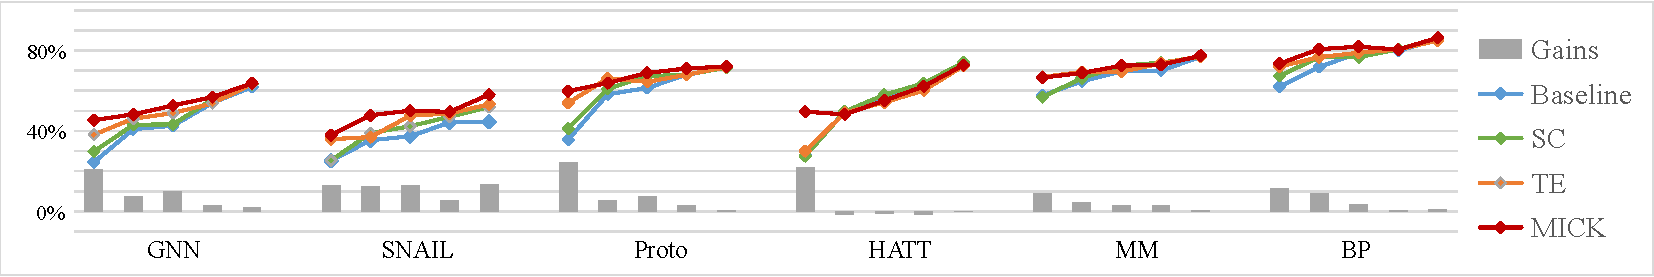
\includegraphics[width=\linewidth]{new51.pdf}
		%\caption{fig1}
	} \\
	\subfigure[5-way 5-shot]{
		\centering
		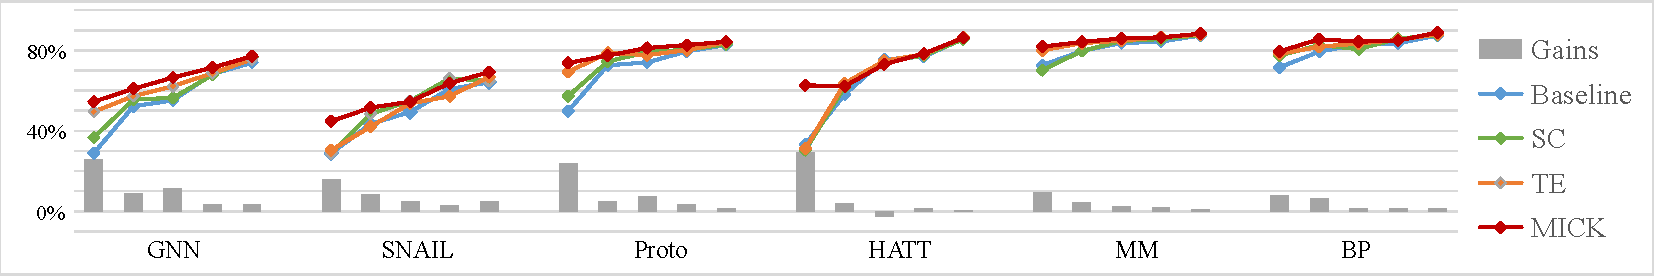
\includegraphics[width=\linewidth]{new55.pdf}
		%\caption{fig2}
	} \\%
	\subfigure[10-way 1-shot]{
		\centering
		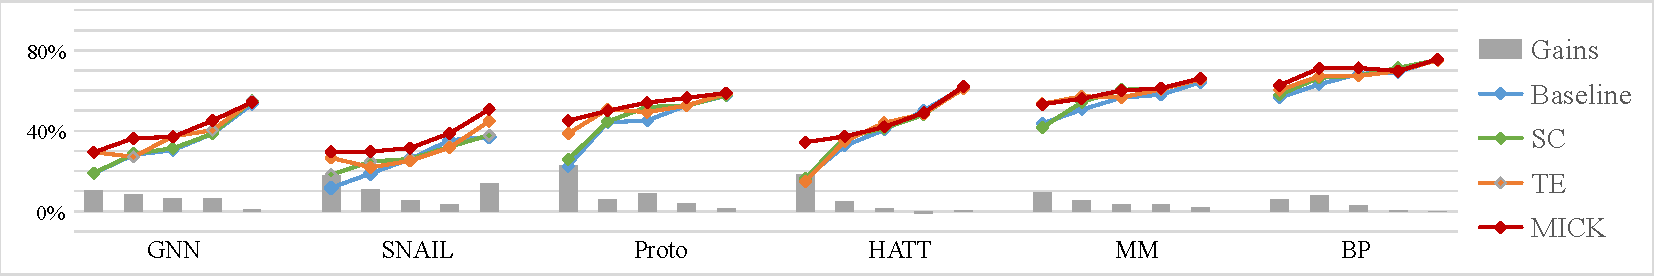
\includegraphics[width=\linewidth]{new101.pdf}
		%\caption{fig2}
	} \\
	\subfigure[10-way 5-shot]{
		\centering
		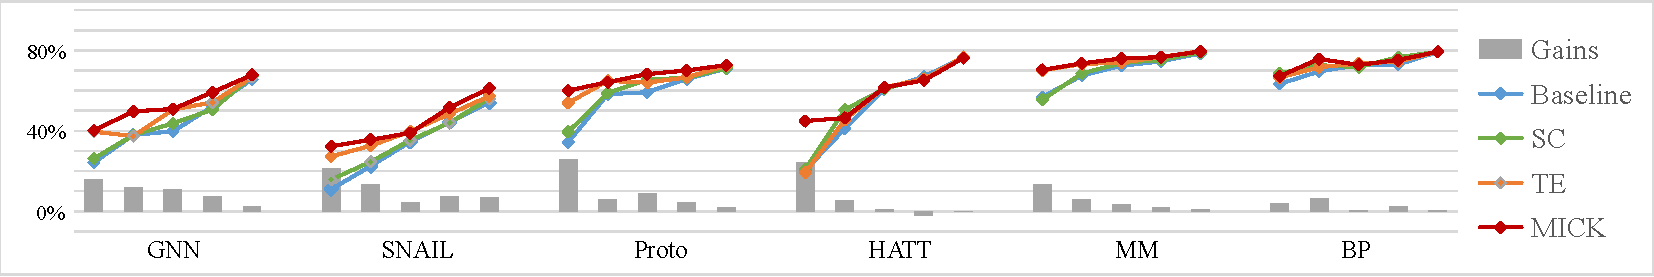
\includegraphics[width=\linewidth]{new105.pdf}
		%\caption{fig2}
	}%
	%\includegraphics[width=0.49\linewidth]{full_results.pdf}
	%%\caption{fig1}
	%}%
	%\subfigure[5-way 5-shot]{
	%\centering
	%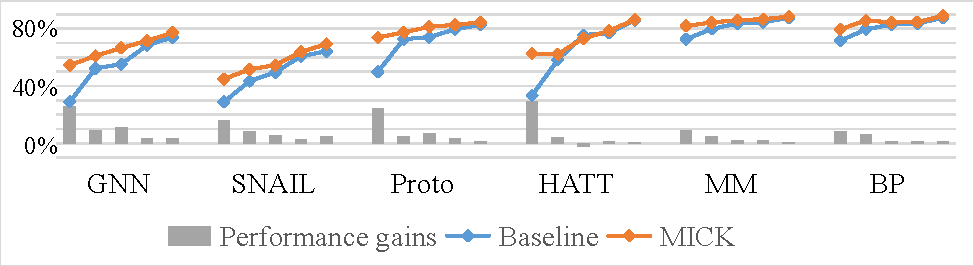
\includegraphics[width=0.49\linewidth]{55.pdf}
	%%\caption{fig2}
	%} \\%
	%\subfigure[10-way 1-shot]{
	%\centering
	%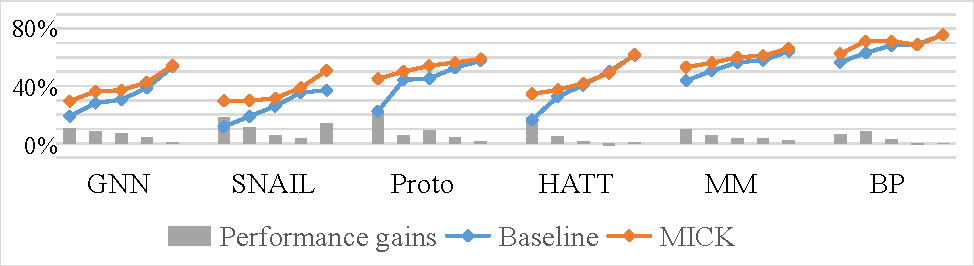
\includegraphics[width=0.49\linewidth]{101.pdf}
	%%\caption{fig2}
	%}%
	%\subfigure[10-way 5-shot]{
	%\centering
	%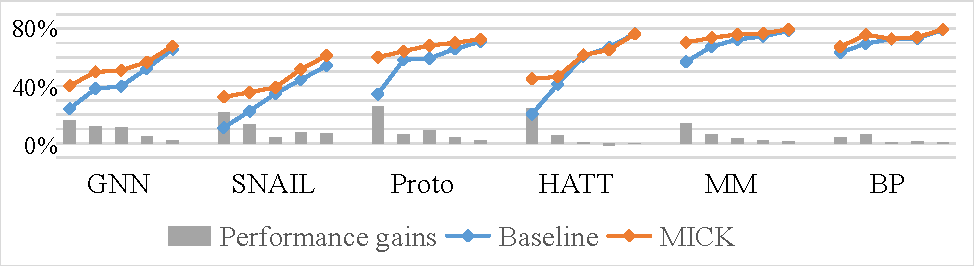
\includegraphics[width=0.49\linewidth]{105.pdf}
	%%\caption{fig2}
	%}%
	
	\centering
	\caption{Classification accuracy on FewRel validation set %with training data shrunken 
		under $N$-way $K$-shot configurations. Gains is the difference between MICK accuracy and baseline accuracy.
		For each group, from the left to the right, training data is shrunken to 0.22\%, 1.00\%, 2.23\%, 7.00\%, and 100.00\% of full training set size, respectively. For each shrunken training set, we apply baseline models and models with SC (Support Classifier individually), TE (Task Enrichment individually) and the whole MICK framework. Proto, HATT, MM, and BP stand for Prototypical Networks, Proto-HATT, MLMAN, and Bert-Pair, respectively.}
	\label{fig:analysis}
\end{figure*}


\subsection{Results and Analysis}
\label{results}
%\KZ{Put more analysis in this section. Make more observation and explain
%things more thoroughly.}
Here, we show the experimental results and analyze them from different aspects.

\subsubsection{With small training data}
To show the effectiveness of our MICK framework under small training data,
we apply it on each baseline model on
(1) FewRel dataset with training set shrunken to different extents, and (2) our proposed TinyRel-CM dataset.

\begin{table*}[th]
\centering
\small
\caption{Classification accuracy (\%) on TinyRel-CM dataset under
	$N$-way $K$-shot configuration.
	% For each cell, $K$=5, 10, and 15 from the top row to the bottom row. 
	D, S, F, and U stand for Disease, Symptom, Food, and nUtrient, respectively.
	Proto, HATT, MM, and BP stand for Prototypical Networks, Proto-HATT, MLMAN, and Bert-Pair, respectively.
	Gray numbers indicate the accuracy is lower than baseline.}
%Meta Networks, SNAIL, GNN, SNAIL and Proto-HATT require the number of classes while training and testing to be equal. So a model is trained with N way tasks to perform N way tests. For SNAIL, the number of instances per relation while training and testing need to be equal. So a model is trained with K shot tasks to perform K shot test tasks.}
\label{FRMresult}
\begin{tabular}{|c|c|cccccc|cccccc|}
\hline
\textbf{Method} & &\multicolumn{6}{c|}{\emph{Baseline}} &\multicolumn{6}{c|}{\emph{+SupportClassifier}} \\ \hline
&\textbf{Group} & D-D & D-S & D-F & D-U & F-U & S-F& D-D & D-S & D-F & D-U & F-U & S-F\\
&\textbf{(N)} & (5) & (2) & (6) & (6)& (2) & (6)& (5) & (2) & (6) & (6)& (2) & (6)\\ \hline
%\multirow{3}{*}{MetaN}      &&&&&& &&&&&& &&&&&& &&&&&&\\
% &&&&&& &&&&&& &&&&&& &&&&&& \\
%&&&&&& &&&&&& &&&&&& &&&&&& \\ \hline
\multirow{3}{*}{GNN}   & (K=~5~)   & 24.04&53.62 &34.15 &38.90 & 54.60& 32.45 &25.71&57.12&33.11&40.23&\textcolor[rgb]{0.45,0.45,0.45}{53.20}&34.51 \\
 & (K=10) & 26.05& 53.73&37.54 &44.02 &\textbf{55.53} &35.45 &\textbf{27.96}&57.35&37.44&43.87&\textcolor[rgb]{0.45,0.45,0.45}{54.85}&\textbf{38.39} \\
 & (K=15) & 26.94& 54.30&38.36 &45.12 &55.45 &37.43 &\textbf{28.36}&61.25&39.18&47.57&\textcolor[rgb]{0.45,0.45,0.45}{55.10}&\textbf{40.37}\\ \hline
\multirow{3}{*}{SNAIL}
 & (K=~5~) &21.74 & 50.00 &17.78 &25.98 & 47.96& 25.38     &23.64&53.90&27.28&27.60&53.15&25.88\\
  & (K=10) & 19.49 & 53.57&27.55 &22.96 &51.63 &22.51      &23.98&56.65&27.76&30.10&54.60&26.10 \\
 & (K=15) & 21.94& 51.62&20.03 &18.21 &50.33 &21.38         &23.12&\textbf{57.40}&27.72&31.43&\textbf{56.35}&25.40\\ \hline
\multirow{3}{*}{Proto}      & (K=~5~)  & 30.03&63.27 &31.35 &33.95 & 54.99& 26.97 &28.99 &\textbf{69.56} &33.57 & 43.78&56.49 &36.81\\
 & (K=10) & 31.68& 67.22&34.09 &36.27 &56.78 &29.18 &32.35 &\textbf{72.54} &36.10 & 47.78& 58.13&39.04\\
 & (K=15) & 33.80& 70.29&34.57 &37.41 &57.03 &29.72 &34.82 &\textbf{72.79} &36.96 &\textbf{50.03} &\textbf{ 60.09} &40.09\\ \hline

% D-D | D-S | D-F | D-U | F-U | S-F %
\multirow{3}{*}{HATT}
 & (K=~5~) &29.67&59.27&40.13&40.19&65.20&41.67  % baseline	5
&36.39&71.45&40.83&\textbf{54.17}&70.09&43.33 \\% cls + data  5
% -------
 & (K=10) &34.50&59.77&39.17&48.33&67.50&43.57  % baseline    10
&40.10&\textbf{71.24}&45.34&50.83&73.33&\textbf{49.17} \\% cls + data  10
% -------
 & (K=15) &39.01&63.75&37.41&\textbf{56.67}&66.25&37.13  % baseline	15
&43.05&77.09&44.17&\textcolor[rgb]{0.45,0.45,0.45}{51.67}&\textcolor[rgb]{0.45,0.45,0.45}{63.75}&45.92  % cls			15
\\% cls + data  15
\hline

\multirow{3}{*}{MM}   & (K=~5~)     &31.22 &60.58 &44.97 &47.11 &61.04 &44.78 &33.48 &62.34 & \textcolor[rgb]{0.45,0.45,0.45}{44.93}&49.49 &62.40 &45.90\\
 & (K=10) & 36.66&64.96 &49.44 &52.49 &66.68 &50.57 &38.89 & 67.30& 50.09& 54.09&68.39 &50.77\\
 & (K=15) & 40.65&68.14 &52.44 &56.00 &70.32 &53.13 &43.05 & 69.41&53.82 &57.23 &72.02 & \textcolor[rgb]{0.45,0.45,0.45}{52.87}\\ \hline
\multirow{3}{*}{BP}  & (K=~5~)    & 23.61&53.48 &46.02 &42.03 & 54.17& 46.18&   24.60 &\textcolor[rgb]{0.45,0.45,0.45}{53.98}&50.49 &\textbf{43.28}&\textbf{63.33}&48.75 \\
 & (K=10) & 24.17& 56.95&49.52 &44.37 &59.72 &48.96 &26.69&\textcolor[rgb]{0.45,0.45,0.45}{55.05} &53.60 &\textbf{46.13}&\textbf{66.70} &51.63  \\
 & (K=15) & 25.80& 54.15&50.38 &45.16 &59.33 &48.78 &27.29 &56.65 &54.22&\textbf{47.81} &67.55 &52.48 \\ \hline
%\multirow{3}{*}{BP2}      & \emph{K=~~5} & 21.83&52.52 &28.73 &30.68 & 54.69& 27.79 &&&&&& &&&&&& &&&&&&\\
%& \emph{K=10} & 22.15& 53.34&32.15 &34.52 &55.20 &30.95 &&&&&& &&&&&& &&&&&&\\
%& \emph{K=15} & 21.56& 54.83&33.74 &36.95 &55.99 &33.00 &&&&&& &&&&&& &&&&&&\\ \hline
%\hline

\textbf{Method} & & \multicolumn{6}{c|}{\emph{+TaskEnrich}} &\multicolumn{6}{c|}{\emph{+SupportClassifier\&TaskEnrich}} \\ \hline
& \textbf{Group} & D-D & D-S & D-F & D-U & F-U & S-F& D-D & D-S & D-F & D-U & F-U & S-F\\
& \textbf{(N)} & (5) & (2) & (6) & (6)& (2) & (6)& (5) & (2) & (6) & (6)& (2) & (6)\\ \hline
\multirow{3}{*}{GNN}
 & (K=~5~) & 24.59&\textcolor[rgb]{0.45,0.45,0.45}{51.20}&\textcolor[rgb]{0.45,0.45,0.45}{33.28}&40.76&54.62&35.36 &\textbf{26.02}&\textbf{66.22}&\textbf{37.48}&\textbf{44.47}&\textbf{55.02}&\textbf{37.13} \\
 & (K=10) &26.85&56.05&37.56&44.90&\textcolor[rgb]{0.45,0.45,0.45}{54.12}&37.69 &27.66&\textbf{58.75}&\textbf{37.88}&\textbf{45.15}&\textcolor[rgb]{0.45,0.45,0.45}{53.42}&37.85 \\
 & (K=15) &27.71&58.55&40.42&49.43&56.35&40.13 &27.40&\textbf{70.10}&\textbf{43.25}&\textbf{51.40}&\textbf{56.45}&40.03 \\ \hline
\multirow{3}{*}{SNAIL}
 & (K=~5~) &22.43&53.95&25.17&\textbf{29.05}&51.30&27.27&\textbf{24.64}&\textbf{58.55}&\textbf{28.57}&27.08&\textbf{53.30}&\textbf{27.88} \\
 & (K=10) &22.79&\textcolor[rgb]{0.45,0.45,0.45}{51.98}&\textbf{30.67}&\textcolor[rgb]{0.45,0.45,0.45}{22.13}&53.15&23.03         &\textbf{27.38}&\textbf{57.12}&\textbf{27.85}&\textbf{33.50}&\textbf{55.60}&\textbf{30.52} \\
 & (K=15) &\textcolor[rgb]{0.45,0.45,0.45}{21.54}&53.10&20.77&\textbf{20.35}&52.00&23.30     &\textbf{23.84}& 56.70&\textbf{30.63}&\textbf{35.75}&54.30&\textbf{30.43} \\ \hline

\multirow{3}{*}{Proto}
 & (K=~5~) &31.40 &69.22 &32.13& 34.22&55.34&30.34&\textbf{31.50} &68.79 &\textbf{34.36} & \textbf{44.76} &\textbf{57.43}&\textbf{40.36} \\ 
 & (K=10) &34.80 &72.34 &34.51&36.58&57.29&33.81&\textbf{35.45} &71.37 &\textbf{37.11} & \textbf{48.28}&\textbf{58.71}&\textbf{43.55} \\
 & (K=15) &36.97 &71.62 &35.76 &37.79 &57.74&34.49&\textbf{38.28} &72.62 &\textbf{37.90} &49.58 &60.00&\textbf{44.97} \\ \hline

\multirow{3}{*}{HATT}
 & (K=~5~) &33.70&67.50&41.67&43.33&65.62&\textcolor[rgb]{0.45,0.45,0.45}{38.33} &\textbf{38.21}&\textbf{75.00}&\textbf{46.67}&49.17&\textbf{73.75}&\textbf{44.17} \\
 & (K=10) &38.98&68.75&40.13&48.75&\textcolor[rgb]{0.45,0.45,0.45}{60.92}&46.67  % data        10
&\textbf{44.45}&70.23&\textbf{49.37}&\textbf{51.67}&\textbf{75.00}&44.47 \\
 & (K=15) &40.39&72.31&43.84&\textcolor[rgb]{0.45,0.45,0.45}{55.83}&70.51&43.33  % data		15
&\textbf{49.61}&\textbf{80.41}&\textbf{44.33}&\textcolor[rgb]{0.45,0.45,0.45}{55.81}&\textbf{72.58}&\textbf{49.17} \\ \hline

\multirow{3}{*}{MM}
 & (K=~5~) &36.05 & \textbf{64.98}& 45.24&50.03 &61.34 & 46.82&\textbf{38.17} &64.68 & \textbf{45.32}& \textbf{51.30}& \textbf{64.24}& \textbf{48.34} \\
 & (K=10) &42.04 & \textbf{70.02}& \textbf{50.83} &54.85 &67.57 &52.47&\textbf{44.89} &69.93 & 50.75& \textbf{56.60}& \textbf{70.79} &\textbf{53.69} \\ 
 & (K=15) &46.55& 71.95&54.18 &58.19 &72.01 &55.28&\textbf{49.23} & \textbf{72.41}& \textbf{54.25}& \textbf{59.67}& \textbf{74.58}& \textbf{56.67} \\ \hline

\multirow{3}{*}{BP}
 & (K=~5~) &25.25&\textbf{59.52}&48.49&\textcolor[rgb]{0.45,0.45,0.45}{40.32}&55.73&48.68 &\textbf{26.87}&58.35&\textbf{52.54}&\textcolor[rgb]{0.45,0.45,0.45}{39.48}&62.52&\textbf{49.95} \\
 & (K=10) &27.54&61.48&51.11&\textcolor[rgb]{0.45,0.45,0.45}{44.33}&60.15&51.56 &\textbf{28.19}&\textbf{62.32}&\textbf{55.86}&\textcolor[rgb]{0.45,0.45,0.45}{43.25}&66.38&\textbf{52.92} \\
 & (K=15) &28.29&\textbf{63.98}&52.18&47.32&61.02&53.36 &\textbf{29.25}&63.15&\textbf{57.60}&\textcolor[rgb]{0.45,0.45,0.45}{43.26}&\textbf{68.83}&\textbf{54.16} \\ \hline
\end{tabular}
\end{table*}


Figure \ref{fig:analysis} shows the performance comparison between baseline models and our framework given different amount of training data on FewRel dataset. 
Each subgraph contains 6 groups, one group for each baseline model. For each group, the training data size increases from the left to right. 
Here, we focus on the blue curves which present baseline accuracies, the red curves which present the MICK enhanced model accuracies, and the gray bars which present the performance gains that MICK brings.
As is illustrated, performance of models deteriorates with the decrease of training data size. For example, the prototypical networks achieves 57.53\% accuracy with full training data under 10-way 1-shot test tasks, but performs poorly with 22.30\% accuracy given only 0.22\% of full training data.
Our framework fits in situations where only small training data is available. As is shown in Figure \ref{fig:analysis}, with our methods, the less the training data, the more improvement the model tends to gain. This indicates the effectiveness of our framework under extremely small training data. While our methods only improve prototypical networks by 1.27\% accuracy with full training data under 10-way 1-shot test tasks, it leads to 22.74\% improvement given 0.22\% of full training data.
%When the input sentence contains multiple relation classes, model performance drops (by 14.14\% under 2.23\% full FewRel training data under 5-way 5-shot tasks using MLMAN). 

Table \ref{FRMresult} shows the experimental results on the TinyRel-CM dataset.
Our framework considerably improves model performance in most cases.
Strong baselines on FewRel dataset such as Bert-Pair do not perform well, partially because the TinyRel-CM dataset is more verbal and informal, thus quite distinct from BERT-Chinese's pretraining data (Chinese Wikipedia).

On both datasets, when the input sentence contains multiple relation classes, model performance drops. E.g., under 2.23\% full FewRel training data under 5-way 5-shot tasks using MLMAN, classification accuracy on relation class \emph{mother} decreases by 14.14\% when \emph{spouse} or \emph{child} appears as interference.

\subsubsection{With sufficient training data}

We use full training data from FewRel dataset and apply MICK framework on each baseline model.

Here, we focus on the rightmost blue points, red points and gray bars of each group in \figref{fig:analysis}, which present the baseline performance, MICK performance and performance gains brought by MICK under full FewRel training data. As is shown in \figref{fig:analysis}, on full FewRel dataset, in most cases, our framework achieves better performance than baseline models.
The framework brings more improvement for relatively poor baselines such as GNN and SNAIL (about 5\% accuracy) than strong baselines such as MLMAN and Bert-Pair (about 1\% accuracy). This is because our framework aims to help models learn better and doesn't change the core part of the models. Full training data is sufficient for strong baselines to train a good model, leaving limited room for improvement. 
%However, we show in \figref{fig:analysis} that by cutting down the training data size, the advantage of our framework is apparent.



% \subsubsection{FewRel dataset with reduced training data}
%Table \ref{FewRelval} shows the experimental results on the FewRel dataset. We either keep the original training set or shrink the training set to different extents and test on the validation set. Table \ref{FewRelval} illustrates the strength of our framework and data augmentation method since performance gains are attained in most cases. While the MSI framework keeps helping models to leaner better, data augmentation tends to be more effective when training data is quite limited.
%Figure \ref{fig:analysis} shows the performance gains on MLMAN using MSI framework and data augmentation. The less the training data, the more improvement the model gains, indicating that the MSI framework and data augmentation method's effectiveness under extremely limited training data.




\subsubsection{Ablation tests}

Here, we focus on the individual effects of support classifier and task enrichment on baseline models. %We facilitate baseline models with either MSI framework or data augmentation and compare the performance with both baseline models and models with

As is shown in Figure \ref{fig:analysis} and Table \ref{FRMresult}, in most cases, either adding support classifier or task enrichment improves performance for baseline models.
%and either removing support classifier or data augmentation leads to performance decrease from the models trained with both methods.
This illustrates that both support classifier and task enrichment contribute to better performance.

On FewRel dataset, we focus on the green and orange curves in \figref{fig:analysis}, which present the accuracies of applying support classifier or task enrichment individually.
% Support classifier
Support classifier generally brings more performance gains when less training data is given. This is because with small training data, baseline models fail to extract adequate knowledge while the support classifier helps with the knowledge learning process.
In some rare cases such as SNAIL under 5-way 1-shot and 5-way 5-shot scenarios with 0.22\% training data, adding support classifier leads to not much improvement. 
This is because support classifier guides models to extract more knowledge from very limited resources, while the extractable knowledge is restricted by the training set size and some of the knowledge is even useless.
Support classifier improves poor baselines such as GNN and SNAIL to a larger extent than strong ones such as MLMAN and Bert-Pair because the support classifier makes up for the insufficient learning ability for poor models while is icing on the cake for strong models. %with sufficient training data.

%TE
Task enrichment is much more helpful than support classifier under small training data (when training data is shrunken to less than 1.00\%). This is because task enrichment compensates for the lack of learning sources of basic knowledge such as basic rules and grammar when training data is quite limited.
Improvement of task enrichment is also more obvious on poor baselines than strong ones. Since poor models fail to master some of the basic knowledge brought in original training data, the introduction of cross-domain data not only brings extra basic knowledge but also helps models to master knowledge in original training data by providing more related data.
%provides more learning resources and help the models learn better about basic knowledge. 

Applying both support classifier and task enrichment achieves best performance in most cases, because the two methods complement each other. Support classifier extract useful information from original training data and cross-domain data, and task enrichment provide extra sources for the support classifier. %knowledge from both original training set and cross-domain data are fully extracted. 
In some cases, although adding either support classifier or task enrichment does not affect much, applying them together leads to a great improvement (e.g., HATT under 0.22\% training data).
%When applied together, support classifier leads to more gains when applied on task enriched models. Because cross-domain data may lead to noise while support classifier helps to choose what to learn.

%Both support classifier and task enrichment bring more performance gains for poor baselines such as GNN and SNAIL than strong ones such as MLMAN and Bert-Pair. 
%Support classifier is more powerful on poor models because the support classifier makes up for the insufficient learning ability for poor models while is icing on the cake for strong models with sufficient training data.
%Improvement of task enrichment is also more obvious on poor baselines than strong ones. Since poor models fail to master basic knowledge such as basic rules and grammar, the introduction of cross-domain knowledge provides more learning resources and help the models learn better about basic knowledge. While for strong models that already learn basic knowledge well, cross-domain task enrichment may bring in noise because of distinct data distributions. This is why sometimes task enrichment brings negative gains.
%stable on strong baselines while fluctuates on poor ones. This reflects the unstableness of poor baselines. With defects in learning ability, supplementary data brings harder tasks and may confuse poor models, and this is why sometimes data augmentation brings negative gains.

On TinyRel-CM dataset (\tabref{FRMresult}), %the improvement is more obvious with either support classifier or task enrichment than on FewRel dataset because of more room for progress.
task enrichment brings about similar improvements for all baselines due to small training data. Support classifier leads to more performance gains than task enrichment individually,
indicating TinyRel-CM dataset is more challenging (the relation classes are much more similar than FewRel dataset) and baseline models fail to extract sufficient useful knowledge.
%indicating model's learning ability is more essential than extra knowledge. 
Although task enrichment brings not much improvement or even negative effects in some cases, adding support classifier simultaneously tend to raise the accuracy to a large extent (up to 10\%). 
The reason is that with insufficient learning ability %(including strong baselines such as MLMAN and Bert-Pair under small data size \KZ{On the one hand you said insufficient learning ability, on the other
%hand you said strong baseline, contradiction?}),
(although baselines such as MLMAN and Bert-Pair are relatively strong, their learning ability is still insufficient with small training data),
cross-domain data alone sometimes introduces
noise and thus confuses the model. But with the additional support classifier
that improves learning ability, models are able to learn more useful
knowledge from cross-domain data.
%This is because with poor learning ability (although baselines such as MLMAN and Bert-Pair are strong on FewRel dataset, their learning ability is still unsatisfying under such small data size), cross-domain data sometimes make things tougher and may confuse the model, while with support classifier which improves learning ability, models are able to learn useful knowledge from cross-domain data.

On %both FewRel dataset (\tabref{FewRelvalAll}) and
TinyRel-CM dataset (\tabref{FRMresult}), few cases occur where adding both support classifier and task enrichment performs worse than adding only one of them
(e.g., Bert-Pair under group D-U, and prototypical networks under group D-S in TinyRel-CM dataset).
The main reason is that while adding the support classifier helps models learn more and better, the model occasionally tend to pay excessive attention to the distinctive distribution of the cross-domain data.
As is shown in the corresponding results, in the vast majority of cases, while adding support classifier on baseline models raises accuracy, adding support classifier on task enriched models brings less improvement or even bad effect. This indicates stronger learning ability owing to the support classifier, and the distraction caused by cross-domain data.

\begin{table}[ht]
	\centering
	\small
	\caption{Human evaluation result on TinyRel-CM dataset under 5-shot scenario.}
	\label{human}
	\begin{tabular}{|c|cccccc|}
		\hline
		\textbf{Group} & D-D & D-S & D-F & D-U & F-U & S-F \\
		\textbf{(N)} & (5) & (2) & (6) & (6) & (2) & (6) \\ \hline
		\textbf{Acc(\%)} & 92.65 &96.53 & 86.93 & 91.77 & 96.71& 84.97\\ \hline
	\end{tabular}
\end{table}

\subsubsection{Dataset analysis}
Our TinyRel-CM dataset is a challenging task.
We human evaluate the dataset and results are illustrated in Table \ref{human}.
During the human-evaluation process, under $N$-way $K$-shot scenario, we provide instances of $N$ relation classes with $K$ instances per relation class. We use labels $1$ to $N$ to name the relation classes instead of their real names. A person is required to classify a new coming instance into one of the $N$ classes. 
We only evaluate the TinyRel-CM dataset under 5-shot scenarios because 10-shot and 15-shot tasks are too easy for human.
Three volunteers participated in the human evaluation process and we take the average accuracy as the final result.

Comparing Table \ref{FRMresult} and Table \ref{human}, the performance of state-of-the-art models is still far worse than human performance, indicating the TinyRel-CM dataset is a challenging task.


%Our TinyRel-CM dataset is more challenging than FewRel dataset.
%The TinyRel-CM dataset has two major difficulties.
%One is the tiny training data size. As is shown in \figref{fig:analysis}, as the training data shrinks, the performance of each model drops evidently. This indicates the less the training data, the more challenging the task becomes.
%
%The other difficulty is that, in TinyRel-CM dataset, given any test task, head and tail entity types of each relation class are the same. This makes the TinyRel-CM dataset more challenging than FewRel dataset even with similar amount of training data.
%Comparing \tabref{FRMresult} and \figref{fig:analysis}, taking baseline MLMAN as an example, MLMAN achieves over $80\%$ accuracy under 5-way 5-shot configuration with $2.23\%$ of full FewRel training data (20 classes with 50 instances per class), while only $31.22\%$ accuracy under 5-way 5-shot configuration (D-D group) with TinyRel-CM dataset (22 classes with 50 instances per class as training set).
%
%To confirm this issue, we choose relation class \emph{mother}, the head and tail entity types of which are \emph{PERSON1} and \emph{PERSON2}, in FewRel dataset as a sample for further analysis. We compute two accuracies: (1) Distinct entity type accuracy: classification accuracy of relation class \emph{mother} without any other candidate relation classes whose target entity types are \emph{PERSON1} and \emph{PERSON2}, and (2) Same entity type accuracy: classification accuracy of \emph{mother} where \emph{spouse} or \emph{child} is among the candidate classes in the same task. We do this analysis under three typical baseline models: prototypical networks, MLMAN and Bert-Pair. We conduct 5-way 5-shot test configuration under $2.23\%$ full training data (20 classes with 10 instances per class). Results are shown in \tabref{etypeanalysis}.  As is illustrated, the accuracy of \emph{mother} accompanied by \emph{spouse} or \emph{child} is much lower than the accuracy of \emph{mother} without same-entity-type classes, indicating shared target entity types among candidate classes brings challenge to models.
%Only two relation classes with the same target entity types raise such difficulty, not to mention the TinyRel-CM dataset where all candidate classes have common target entity types.
%
%\begin{table}[ht]
%\centering
%\small
%\caption{5-way 5-shot classification accuracy (\%) on relation class \emph{mother} in FewRel dataset.
%	Etype stands for Entity type.
%	%Distinct etype represents classification accuracy with other candidate classes that have distinct target entity types with \emph{mother}.
%	%Same etype represents classification accuracy where some candidate classes share same target entity types with \emph{mother}.
%	Proto, MM, and BP stand for Prototypical Networks, MLMAN, and Bert-Pair, respectively.}
%\label{etypeanalysis}
%\begin{tabular}{|c|p{56pt}<{\centering}|p{56pt}<{\centering}|}
%\hline
%\textbf{Method} &\textbf{Distinct Etype} & \textbf{Same Etype} \\ \hline
%Proto & 77.91 & 63.39 \\
%MM & 86.84 & 72.70 \\
%BP & 96.89& 54.67 \\ \hline
%\end{tabular}
%\end{table}

